\section{Introduction}

This guide is aimed at helping those people who have day-to-day responsibility
for supervising a placement student from the University of Ulster.

Your student can fill in your details in his or her placement record, using
OPUS at \url{\opusurl}. At that point you will be sent a username and
password to access the system; provided an email address was specified when
your details were added.

This guide explains what this account can be used for, and whether you will want
to use it.

\subsection{Multiple Accounts}

Please note that you may already have a user on OPUS, in which case that account
probably has a different purpose (for example, to be used to recruit students in the
first place). You should continue to keep the credentials for that account in addition
to your supervisor account.

If you supervise several students you may find you receive several accounts for use
in supervising these students. Please retain all the credentials for each account
until the placements are complete.

\section{Getting Started}.

If you have not already got an account on the OPUS then please speak to your normal contact
for placement within the University, or email
% @todo add an email address here
to have an account made for you.

When you have your login details, you can login at \url{\opusurl}.

When you login, you will see something like the following
\begin{figure}[htb]
\begin{center}
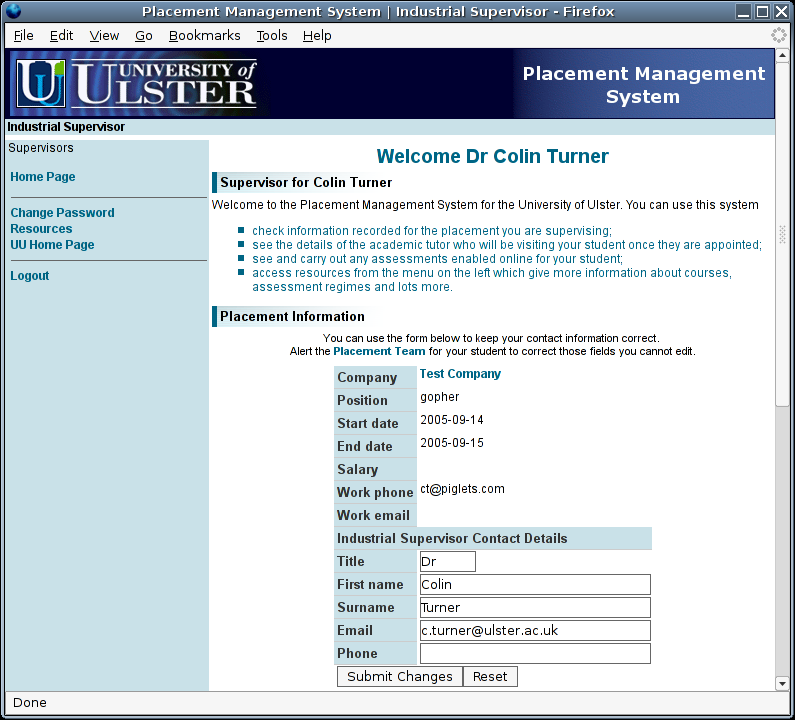
\includegraphics[scale=0.25]{png/supervisor_guide1.png}
\end{center}
\caption{Your home page (top part)}
\end{figure}
On the left hand side you will see a menu. 
At any time clicking on ``Home Page'' will return you here. The other menu
items in turn are

\begin{description}
\item[Change Password] allows you to alter the preconfigured password;
\item[Resources] provides a large collection of documents to guide you;
\item[UU Home Page] takes you the main university home page;
\item[Logout] logs you out from the system.
\end{description}

At any time, clicking on the link for the ``Help Directory'' at the bottom of the page
will provide you with details on the staff who are most likely to be
able to help with your enquiries.

\section{What can you do?}

Here is a summary of what this account offers you.

\subsection{Placement Information}

As you can see, the home page shows some information about the placement. Some of
this cannot be edited for important operational reasons, but you can contact the
staff in the help directory if you need it to be changed.

You will also see your own contact details, which naturally you can edit for your
convenience.

\subsection{Academic Tutor}

Students on placement will also be allocated an academic tutor, although sometimes
this takes some time after the initial placement. If the academic tutor is
appointed you will see their details on-screen.

\begin{figure}[htb]
\begin{center}
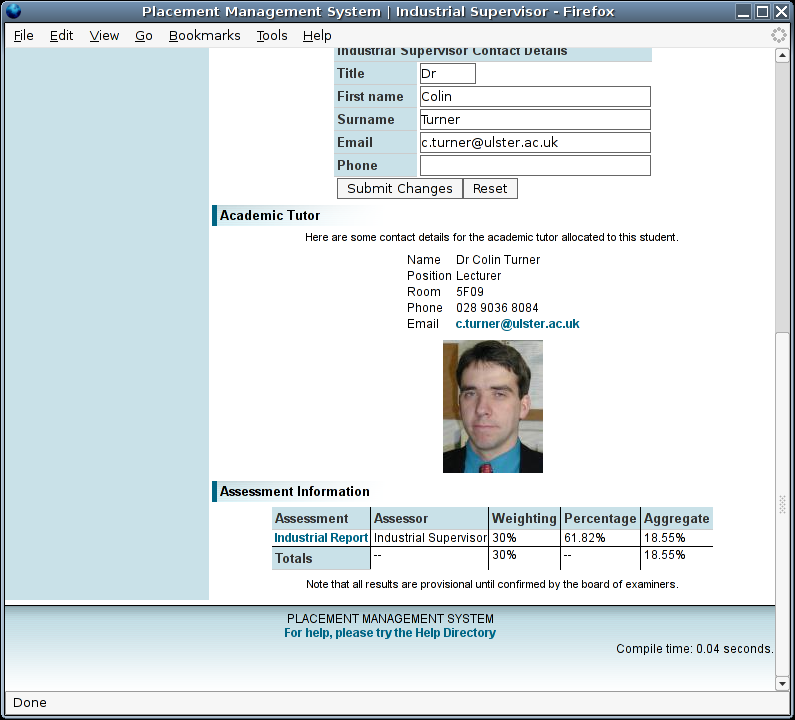
\includegraphics[scale=0.25]{png/supervisor_guide2.png}
\end{center}
\caption{Your home page (bottom part)}
\end{figure}

Usually this staff member will visit the student during the placement, and in any case
provides another important contact if you have any worries or concerns.

\subsection{Assessment}

You may also be invited to file assessments for the student on-line, and if so, the
assessments will be shown on the screen. Simply click on the assessment name to fill
in the assessment at the appropriate time.

\subsection{Help Directory}

Click on the help directory at the bottom of the screen to find out who is available
to help you with any queries you may have about the placement.

\subsection{Resources}

When you click on \emph{resources} on the left, you will be shown a list of documents
that may help you managing this placement.
